\documentclass[main.tex]{subfiles}
\begin{document}

\section{Correspondance of FASIII and Relative FASIII scores}
\label{appendix:FASIII_RelFAS}

% \begin{table}[htbp]
% \centering
% \tiny{
% % [Insert your summary statistics table here, as in your original appendix]
% }
% \caption{Summary statistics of all selected variables.}
% \end{table}
% \end{document}

\begin{figure}[htbp]
    \centering
    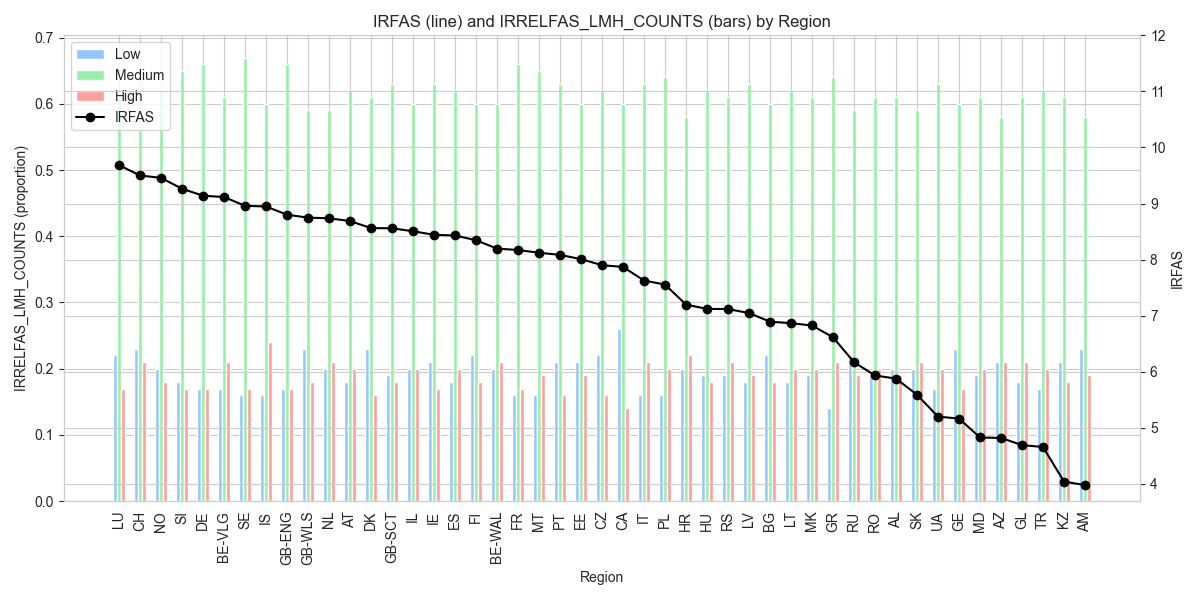
\includegraphics[width=0.8\textwidth]{Report/final_report/pictures/IRFASvsIRRELFAS.png}
    \caption{Comparison of weighted average Family Affluence Score (IRFAS, black line) and the distribution of relative family affluence categories (Low, Medium, High; colored bars) across regions. Regions are ordered by descending IRFAS. The left y-axis shows the proportion of each affluence category, while the right y-axis displays the average IRFAS}
    \label{fig:IRFASvsIRRELFAS}
\end{figure}



\section{Meek's Rules for FCI \cite{ZHANG20081873}}
\label{appendix:Meek_FCI}
\begin{align*}
\mathcal{R}0. &\quad \text{(Unshielded Collider)} \\
&\text{If } X *\!\!-\!\!* Y *\!\!-\!\!* Z,\ \text{and } X \text{ and } Z \text{ are not adjacent, and } Y \notin \text{SepSet}(X, Z), \\
&\text{then orient as } X *\!\!-\!\!> Y <\!\!-\!\!* Z. \\[1ex]
\mathcal{R}1: \quad & \text{If } X \ast\!\!-\!\!\ast Y \circ\!\!-\!\!\ast Z, \text{ and } X \text{ and } Z \text{ are not adjacent, then orient as } X \ast\!\!-\!\!\ast Y \rightarrow Z. \\[1em]
\mathcal{R}2: \quad & \text{If } X \rightarrow Y \ast\!\!-\!\!\ast Z \text{ or } X \ast\!\!-\!\!\ast Y \rightarrow Z, \text{ and } X \ast\!\!-\!\!\circ Z, \\
& \text{then orient } X \ast\!\!-\!\!\circ Z \text{ as } X \ast\!\!-\!\!\ast Z. \\[1em]
\mathcal{R}3: \quad & \text{If } X \ast\!\!-\!\!\ast Y \leftrightarrow Z,\, X \ast\!\!-\!\!\circ M \circ\!\!-\!\!\ast Z,\, X \text{ and } Z \text{ are not adjacent, and } M \ast\!\!-\!\!\circ Y, \\
& \text{then orient } M \ast\!\!-\!\!\circ Y \text{ as } M \ast\!\!-\!\!\ast Y. \\[1em]
\mathcal{R}4: \quad & \text{If } u = (M, \ldots, X, Y, Z) \text{ is a discriminating path between } M \text{ and } Z \text{ for } Y, \\
& \text{and } Y \circ\!\!-\!\!\ast Z; \text{ then if } Y \in \mathrm{SepSet}(M, Z), \text{ orient } Y \circ\!\!-\!\!\ast Z \text{ as } Y \rightarrow Z; \\
& \text{otherwise orient the triple } (X, Y, Z) \text{ as } X \leftrightarrow Y \leftrightarrow Z. \\[1em]
\mathcal{R}5: \quad & \text{For every (remaining) } X \circ\!\!-\!\!\circ Z, \text{ if there is an uncovered circle path } p = (X, M, \ldots, K, Z) \\
& \text{between } X \text{ and } Z \text{ such that } X, K \text{ are not adjacent and } Z, M \text{ are not adjacent,} \\
& \text{then orient } X \circ\!\!-\!\!\circ Z \text{ and every edge on } p \text{ as undirected edges } (-). \\[1em]
\mathcal{R}6: \quad & \text{If } X \ast\!\!-\!\!\ast Y \circ\!\!-\!\!\ast Z \, (X \text{ and } Z \text{ may or may not be adjacent}), \\
& \text{then orient } Y \circ\!\!-\!\!\ast Z \text{ as } Y \rightarrow Z. \\[1em]
\mathcal{R}7: \quad & \text{If } X \circ\!\!-\!\!\circ Y \circ\!\!-\!\!\ast Z, \text{ and } X, Z \text{ are not adjacent, then orient } Y \circ\!\!-\!\!\ast Z \text{ as } Y \rightarrow Z. \\[1em]
\mathcal{R}8: \quad & \text{If } X \rightarrow Y \rightarrow Z \text{ or } X \circ\!\!-\!\!\circ Y \rightarrow Z, \text{ and } X \circ\!\!-\!\!Z, \text{ orient } X \circ\!\!-\!\!Z \text{ as } X \rightarrow Z. \\[1em]
\mathcal{R}9: \quad & \text{If } X \circ\!\!-\!\!Z, \text{ and } p = (X, Y, M, \ldots, Z) \text{ is an uncovered p.d. path from } X \text{ to } Z \\
& \text{such that } Z \text{ and } Y \text{ are not adjacent, then orient } X \circ\!\!-\!\!Z \text{ as } X \rightarrow Z. \\[1em]
\mathcal{R}10: \quad & \text{Suppose } X \circ\!\!-\!\!Z,\, Y \rightarrow Z \leftarrow K,\, p_1 \text{ is an uncovered p.d. path from } X \text{ to } Y, \\
& \text{and } p_2 \text{ is an uncovered p.d. path from } X \text{ to } K. \\
& \text{Let } M \text{ be the vertex adjacent to } X \text{ on } p_1\, (M \text{ could be } Y), \text{ and } A \text{ be the vertex adjacent to } X \text{ on } p_2\, (A \text{ could be } K). \\
& \text{If } M \text{ and } A \text{ are distinct, and are not adjacent, then orient } X \circ\!\!-\!\!Z \text{ as } X \rightarrow Z.
\end{align*}

\noindent
Here, all nodes \( X, Y, Z, M, K, A \in \mathbf{V} \), the set of nodes in the graph.\\
\(\mathcal{R}0\)-\(\mathcal{R}3\) are the inference rules for learning DAGs. \(\mathcal{R}4\) is specific to MAGs with bidirected edges. \(\mathcal{R}5\)-\(\mathcal{R}6\) are irrelevant if the true causal MAG does not contain undirected edges (e.g., no selection bias). \(\mathcal{R}7\) might not be triggered because none of \(\mathcal{R}0\)-\(\mathcal{R}4\) and \(\mathcal{R}8\)-\(\mathcal{R}10\) lead to \( -\!\!\circ \). \(\mathcal{R}8\)-\(\mathcal{R}10\) help convert partially directed edges into directed ones, and together they render an Augmented FCI.


\section{Python causal-learn FCI example}
\label{appendix: python_fci_clean}
\begin{lstlisting}[language=Python]
import numpy as np
import pandas as pd
from causallearn.search.ConstraintBased.FCI import fci
from causallearn.utils.cit import  gsq
from causallearn.utils.GraphUtils import GraphUtils

test_map = {
        "fisherz": fisherz,
        "mv_fisherz": mv_fisherz,
        "gsq": gsq,
        "chi2": chi2,
        "kci": kci
    }


def run_fci(
    data: pd.DataFrame,
    test: str = "gsq",
    alpha: float = 0.05,
    output_dir: str = "graphs"
) -> tuple:
    
    data_array = data.values.astype(np.float32)

    # Run FCI with specified parameters
    graph, edges = fci(
        dataset=data_array,
        independence_test_method=test_map[test],
        alpha=alpha,
        verbose=True
    )

    # Generate visualization
    GraphUtils.to_pydot(graph, labels=data.columns.tolist())
            .write_png(
                os.path.join(output_dir, filename)            )
    return graph, edges
\end{lstlisting}

\section{Python causal-learn FCI }
\label{appendix: python_fci_clean}

\end{document}